% Exposé II.C: cut and volume. Sources: theory/framework.md (II.C), site/sections/05-rank.html, theory/propositions.json.
\subsection{Cut and volume}\label{sec:cut}

\begin{flushright}
\small\itshape Rank lives on cuts and dimension lives in volumes.\\
Count the wrong one and you will compare the wrong things.\\[2pt]
{\upshape\footnotesize a working maxim}
\end{flushright}

At a fixed budget, the narrowest cut of a method's diagram bounds the rank it can reach. The dimension of what it can
reach is a separate count, and the two can move in opposite directions.

\paragraph{In brief}
\begin{itemize}
  \item A method's update rank is bounded by the narrowest cut of its tensor-network diagram. The dimension $d(M)$ of
    what it can reach is its parameter count minus the directions that change nothing.
  \item The two can move in opposite directions. At the budget of LoRA$_8$ on a $4096\times4096$ layer, LoHa$_{4,4}$
    reaches rank $16$ and at least $8{,}159$ fewer dimensions; GraLoRA with $k=2$ reaches rank $16$ at LoRA's
    dimension, with every block capped at rank $4$.
  \item Kronecker sums are LoRA across another cut of the same four-leg tensor, and HiRA is LoRA after
    $X\mapsto W_0\odot X$ (for $W_0$ without zero entries). Such changes of frame keep dimension and move rank.
  \item LoRA respects every change of a layer's coordinates and so reaches the same set of functions after a
    function-preserving rotation of the network; PiSSA, MiLoRA and CorDA splits respect only rotations and uniform
    scalings.
\end{itemize}

PEFT papers usually report a method's expressiveness as a rank and its cost as a parameter count. A third number, the
dimension of the set of weights the method can reach, usually goes unreported.

Draw a method as a network of boxes and wires. The rank of its update is limited by the narrowest place where the
network can be cut in two, so rank is a \emph{cut} invariant. The dimension counts the independent directions in which
the method can move the weights; we call it a \emph{volume} invariant, loosely, since no measure is computed. In
Figure~\ref{fig:rankvol}, several methods raise one while lowering the other.

\begin{figure}[tbp]
  \centering
  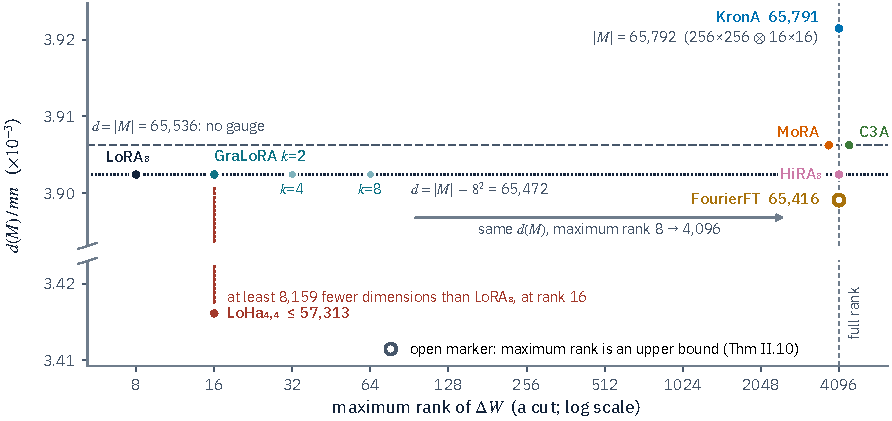
\includegraphics[width=\linewidth]{figures/rankvol}
  \caption{\textbf{Rank is not volume} (\thmref{Theorem}{II.10}, \thmref{Proposition}{II.12}). One $4096\times4096$ layer at the budget of LoRA$_8$ \citep{hu2021lora}, $\lvert M\rvert=8(m+n)=65{,}536$. Each method is placed by the largest rank of $\Delta W$ it can reach (horizontal, logarithmic scale), which is bounded by the narrowest cut of its diagram (\thmref{Theorem}{II.10}), and by its expressive dimension as a fraction of the layer, $d(M)/(mn)$ (vertical, in units of $10^{-3}$, with the axis broken between $3.41$ and $3.90$), from the gauge census of \thmref{Proposition}{II.12}. The dashed line is $d=\lvert M\rvert$, a method without gauge, and the dotted line is $d=\lvert M\rvert-8^2=65{,}472$, the dimension of LoRA$_8$ with its $\GL_8$ gauge. Along the dotted line the maximum rank runs from $8$ for LoRA$_8$, through GraLoRA \citep{jung2025gralora} with $k=2$, $4$ and $8$ blocks (the last two light), to full rank for HiRA$_8$ \citep{huang2025hira}. MoRA \citep{jiang2024mora} and C3A \citep{chen2024parameter} have no gauge and reach full rank; their points coincide and are drawn on either side of the full-rank line. FourierFT \citep{gao2024parameter} loses one dimension for each sampled conjugate pair, and its maximum rank is known only through a bound (open marker). KronA \citep{edalati2022krona} is shown at the factor shapes closest to the budget. LoHa$_{4,4}$ \citep{hyeonwoo2021fedpara}, below the break, sits at the proved upper bound of its dimension: it reaches rank $16$ with at least $8{,}159$ fewer dimensions than LoRA$_8$ (\thmref{Proposition}{II.12}(c)). The parameters behind each point are in \S\ref{app:repro-figures}.}
  \label{fig:rankvol}
\end{figure}

% ----------------------------------------------------------------------------------------------------------------------
\subsubsection{Rank is a cut}\label{sec:cut-rank}

In LoRA every signal crosses the inner wire of dimension $r$ between $A$ and $B$, so $\Delta W=BA$ has rank at most $r$
(Figure~\ref{fig:loraplug}). The argument works for any method drawn as a tensor network (\bgref{B.7}), a string diagram
(\bgref{B.3}) in the symmetric monoidal category $(\FinVect,\otimes)$. Split the boxes into an input side and an output
side, and the network factors through the wires that cross.

\begin{figure}[tbp]
\centering
\begin{tikzpicture}[
  font=\small,
  box/.style={draw=ink, rounded corners=1.5pt, minimum width=8.5mm, minimum height=6.5mm, inner sep=2pt, line width=0.6pt},
  frozen/.style={box, fill=inkgray!14},
  train/.style={box, draw=tide, fill=tide!16, line width=0.8pt},
  wire/.style={draw=ink, line width=0.7pt},
  lab/.style={font=\footnotesize, text=inkgray},
  cutline/.style={draw=seal, line width=1pt, dash pattern=on 3pt off 2pt},
  altcut/.style={draw=inkgray!70, line width=0.6pt, densely dotted}
]
  % (a) the hole left by W_0
  \node[draw=inkgray, dashed, rounded corners=2pt, minimum width=13mm, minimum height=9mm] (hole) at (2.1,0) {};
  \node[lab] at (hole) {hole};
  \draw[wire] (0,0) -- (hole.west);
  \draw[wire] (hole.east) -- (4.2,0);
  \node[lab, anchor=south] at (0.55,0.08) {$V=\R^n$};
  \node[lab, anchor=south] at (3.65,0.08) {$U=\R^m$};
  \node[lab, anchor=north] at (2.1,-1.05) {(a) $W_0$ cut out of a linear layer};
  % (b) the LoRA plug
  \begin{scope}[xshift=5.2cm]
    \node[frozen] (W0) at (0.9,0) {$W_0$};
    \draw[wire] (0,0) -- node[above,lab]{$n$} (W0.west);
    \draw[wire] (W0.east) -- node[above,lab]{$m$} (1.8,0);
    \node at (2.2,0) {$+$};
    \node at (2.6,0) {$s$};
    \node[train] (A) at (4.1,0) {$A$};
    \node[train] (B) at (6.4,0) {$B$};
    \draw[wire] (2.85,0) -- (A.west);
    \draw[wire] (A.east) -- (B.west);
    \draw[wire] (B.east) -- (7.95,0);
    \node[lab, anchor=south] at (3.05,0.08) {$n$};
    \node[lab, anchor=south] at (4.82,0.08) {$r$};
    \node[lab, anchor=south] at (7.1,0.08) {$m$};
    \draw[altcut] (3.4,0.5) -- (3.4,-0.5) node[below, lab]{$n$};
    \draw[altcut] (7.45,0.5) -- (7.45,-0.5) node[below, lab]{$m$};
    \draw[cutline] (5.25,0.62) -- (5.25,-0.62);
    \node[font=\footnotesize, text=seal, anchor=south] at (5.25,0.62) {cut of weight $r$};
    \node[lab, anchor=north] at (4.0,-1.05) {(b) the LoRA plug $W_0+sBA$};
  \end{scope}
\end{tikzpicture}
\caption{\textbf{LoRA as a plug.} (a) Cutting $W_0$ out of a linear layer $y=W_0x$ leaves a hole $V\to U$, with
  $V=\R^n$ and $U=\R^m$. (b) LoRA fills the hole with the frozen box $W_0$ (grey) plus the trainable chain $sBA$ (teal),
  a formal sum, over which rank is subadditive. The dashed cut puts $A$ on the input side and $B$ on the output side and
  crosses one wire of dimension $r$, so $\rk(sBA)\le r$ (\thmref{Theorem}{II.10}). The dotted cuts put both boxes on one
  side and cross an open leg, with weights $n$ and $m$; the minimum over cuts is $\min(n,r,m)$.}
\label{fig:loraplug}
\end{figure}

\begin{theorem}{II.10}{cut-rank bound; standard}
Let $\Gamma$ be a tensor network, evaluated in the symmetric monoidal category $(\FinVect,\otimes)$, with input legs $V$
and output legs $U$. Every wire and open leg is assumed incident to a vertex: insert an identity box on any bare strand,
or equivalently count each bare input--output wire as crossing every cut. A crossing hyperedge (copy spider) contributes
its dimension once. Partition the vertices into $\mathcal I\sqcup\mathcal O$. The weight $w$ of the cut is the product
of the dimensions of the internal wires between the two sides and of the open legs attached on the wrong side (input legs
at $\mathcal O$, output legs at $\mathcal I$). Then
\begin{equation*}
  \rk\llbracket\Gamma\rrbracket\le\min_{\mathrm{cuts}}w,
\end{equation*}
and rank is subadditive over formal sums. The bound refers to a chosen presentation of the network.
\end{theorem}

\paragraph{Numerical check}
No violation in $283$ random networks (Appendix~\ref{app:repro}).

\paragraph{Credit}
String diagrams go back to \citet{xjoyal1991geometry}, and the copy spider (\bgref{B.6}) to the Frobenius algebra of a
basis \citep{xcoecke2013new}. Cut bounds on rank are standard tensor-network reasoning (\bgref{B.8};
\citealp{kolda2009tensor,cichocki2016low}). The PEFT reading is ours.

Without the convention on bare strands, $I_d\otimes BA$ would violate the bound. The bound also depends on the drawing. A
naive expansion of HRA's product of reflections has $2^r-1$ terms, while the telescoping presentation
\begin{equation*}
  R-I=\sum_{k=1}^{r}(H_k-I)\,H_{k+1}\cdots H_r
\end{equation*}
writes $R-I$ as $r$ terms of rank at most one and gives the sharp bound $r$.

\paragraph{Consequences}
For one box, \thmref{Theorem}{II.10} gives the bounds in Table~\ref{tab:cutbounds}. Relative to $W_0$, splitting
initialisations give $\Delta W=BA-B_0A_0$, of rank at most $2r$ (\thmref{Theorem}{II.1}). The Givens bound uses the same
telescoping presentation as HRA, each gate contributing a term of rank at most two, and HiRA's bound factors $W_0$
through a bond of dimension $\rk W_0$.

\begin{table}[t]
  \centering
  \footnotesize
  \caption{Cut bounds of \thmref{Theorem}{II.10} on $\rk\Delta W$ for one $m\times n$ box, with the presentation each
    bound uses.}
  \label{tab:cutbounds}
  \renewcommand{\arraystretch}{1.12}
  \begin{tabularx}{\linewidth}{@{}>{\raggedright\arraybackslash}p{4.6cm}>{\raggedright\arraybackslash}X>{\raggedright\arraybackslash}p{2.6cm}@{}}
    \toprule
    \headrow \textbf{method} & \textbf{presentation used} & \textbf{bound on $\rk\Delta W$}\\
    \midrule
    LoRA family, $BA$ \citep{hu2021lora} & one bond of dimension $r$ & $r$\\
    split initialisations (PiSSA type), relative to $W_0$ & $\Delta W=BA-B_0A_0$, two bonds & $2r$\\
    HRA \citep{yuan2024bridging} & telescoping sum $R-I=\sum_k(H_k-I)H_{k+1}\cdots H_r$ & $r$\\
    Givens circuit with $g$ gates \citep{ma2024parameter} & the same telescoping sum & $2g$\\
    ReLoRA after $K$ phases \citep{lialin2023relora} & formal sum of $K$ LoRAs & $Kr$\\
    GraLoRA \citep{jung2025gralora} & sum of $k^2$ block LoRAs & $kr$\\
    LoHa \citep{hyeonwoo2021fedpara} & Hadamard product through copy spiders & $r_1r_2$\\
    HiRA \citep{huang2025hira} & $W_0$ factored through a bond of dimension $\rk W_0$ & $r\,\rk W_0$\\
    LoKr \citep{yeh2023navigating} & $C\otimes BA$, inner rank $r'$ & $\rk C\cdot r'$\\
    FourierFT with $n_c$ coefficients \citep{gao2024parameter} & sum of real cosine patterns, each of rank $\le2$ &
      $\min(2n_c,m,n)$\\
    MoRA (reshape) \citep{jiang2024mora}, C3A \citep{chen2024parameter}, MPO adapters \citep{xliu2021enabling} & no
      narrow cut & up to full rank\\
    \bottomrule
  \end{tabularx}
\end{table}

\begin{explains}
A large min-cut is necessary for high rank and does not guarantee it. The ``high-rank PEFT'' literature consists of
networks whose min-cut avoids an $r$-dimensional bottleneck. Whether the bound is attained is a separate question, and
attaining it can cost volume.
\end{explains}

% ----------------------------------------------------------------------------------------------------------------------
\subsubsection{Kronecker adapters cut the other way}\label{sec:cut-kronecker}

If $m=m_1m_2$ and $n=n_1n_2$, an $m\times n$ matrix is a tensor with output legs $U_1,U_2$ and input legs $V_1,V_2$
(\bgref{B.10}). LoRA's rank is the rank across $\{U_1U_2\}\mid\{V_1V_2\}$; a sum of $k$ Kronecker products has rank at
most $k$ across $\{U_1V_1\}\mid\{U_2V_2\}$. The two cuts disagree sharply, since $I\otimes I$ is one Kronecker term of
full rank.

\begin{theorem}{II.11}{Kronecker incomparability; the linear algebra is standard, the PEFT reading is new}
Write $\R^m=\R^{m_1}\otimes\R^{m_2}$ and $\R^n=\R^{n_1}\otimes\R^{n_2}$, and view $\Delta\in\R^{m\times n}$ as a 4-leg
tensor. Let $\operatorname{rk}$ be the rank across the cut $\{U_1U_2\}\mid\{V_1V_2\}$ and $\operatorname{rk}_\otimes$
the rank across $\{U_1V_1\}\mid\{U_2V_2\}$. Put
\begin{equation*}
  \kappa_1:=\min(m_1,m_2)\cdot\min(n_1,n_2),\qquad\nu:=\min(m_1,n_1)\cdot\min(m_2,n_2).
\end{equation*}

(a) $\operatorname{rk}_\otimes\Delta\le k$ iff $\Delta=\sum_{i\le k}C_i\otimes D_i$. Every $\Delta$ has
$\operatorname{rk}_\otimes\Delta\le\min(m_1n_1,m_2n_2)$.

(b) $\operatorname{rk}(C\otimes D)=\operatorname{rk}C\cdot\operatorname{rk}D$, while
$\operatorname{rk}_\otimes(C\otimes D)=1$ for $C,D\ne0$. So $\nu$ is the largest rank of a single Kronecker product.

(c) If $u\in\R^m$ and $v\in\R^n$ have Schmidt ranks $\rho_u,\rho_v$ (\bgref{B.12}), then
$\operatorname{rk}_\otimes(uv\T)=\rho_u\rho_v$. A generic rank-one update therefore has Kronecker rank $\kappa_1$. For
aligned splits, $(m_1-m_2)(n_1-n_2)\ge0$, which include equal square splits and every split HF PEFT's factorisation
produces (it puts the smaller factor first on both sides), $\kappa_1=\min(m_1n_1,m_2n_2)$ is the maximal Kronecker rank.

(d) \emph{Incomparability.} For $1\le r<\nu$ and $1\le k<\kappa_1$, the sets $\Mr$ and
$\mathcal K_{\le k}:=\{\Delta:\operatorname{rk}_\otimes\Delta\le k\}$ of unconstrained $k$-term Kronecker sums are
incomparable, for every split. A generic rank-one update lies in the first and not the second, and $C\otimes D$ with
full-rank factors, of Kronecker rank $1$ and rank $\nu$, lies in the second and not the first. For equal square splits
($m=n=N$, all factors $s$), $\kappa_1=\nu=s^2=N$, and $I_N$ is such a product.

(e) \emph{Constrained Kronecker methods.} Let $\Im M\subseteq W_0+\mathcal K_{\le k}$. Then
$\Im\mathrm{LoRA}_r\not\subseteq\Im M$ whenever $k<\kappa_1$, for every pointing of $\mathrm{LoRA}_r$. Give
$\mathrm{LoRA}_r$ its zero-init pointing, with image $W_0+\Mr$. Then $\Im M\not\subseteq\Im\mathrm{LoRA}_r$ iff some
$\theta\in\Im M$ has $\rk(\theta-W_0)>r$. For LoKr, $\Delta W=C\otimes BA$ with $C\in\R^{m_1\times n_1}$,
$B\in\R^{m_2\times r'}$ and $A\in\R^{r'\times n_2}$, put $r'_{\mathrm{eff}}=\min(r',m_2,n_2)$. The maximum rank is
$\min(m_1,n_1)\cdot r'_{\mathrm{eff}}$, attained. So $\Im\mathrm{LoKr}_{r'}\subseteq\Im\mathrm{LoRA}_r$ iff
$r\ge\min(m_1,n_1)\,r'_{\mathrm{eff}}$, and otherwise the two images are incomparable, provided $\kappa_1>1$. In HF PEFT
the second LoKr factor is low-rank only when its rank parameter satisfies $r'<\max(m_2,n_2)/2$; otherwise it is full,
and LoKr is unconstrained KronA, with maximum rank $\nu=\min(m_1,n_1)\min(m_2,n_2)$. On a $768$-wide layer
($24\otimes32$) the maximum rank therefore jumps from $360$ at $r'=15$ to $768$ at $r'=16$. With
\texttt{decompose\_both}, $C$ is also capped at rank $r'$.
\end{theorem}

\paragraph{Numerical check}
Schmidt ranks $(1,3)\to3$, $(2,3)\to6$, $(3,3)\to9$, each with ordinary rank $1$. For the $2\times4$ split of $\R^8$,
$\operatorname{rk}_\otimes(uv\T)=4$, the maximal Kronecker rank there. LoKr with $s=4$, $r'=1$ never exceeds rank $4$,
and at $(m_1,m_2,n_1,n_2)=(2,8,8,2)$ with inner dimension $4$, LoKr never exceeds rank
$4=\min(m_1,n_1)\,r'_{\mathrm{eff}}$ (Appendix~\ref{app:repro}).

\paragraph{Credit}
The rearrangement $\mathcal R(C\otimes D)=\vect C\,\vect D\T$ (\bgref{B.11}) and the nearest-Kronecker-product problem
are due to Van Loan and Pitsianis~\citeyearpar{loan1993approximation}. Kronecker-sum layers entered deep learning with
PHM layers \citep{zhang2021beyond} and Compacter \citep{mahabadi2021compacter}; KronA \citep{edalati2022krona} and LoKr
\citep{yeh2023navigating} brought them to weight updates.

\begin{explains}
Unconstrained Kronecker sums (KronA with full factors, sums of Kronecker terms) are LoRA across a different cut of the
same 4-leg tensor, so calling them higher-rank LoRAs mixes two cuts. With aligned splits, a generic rank-one update needs
the maximal number of Kronecker terms, and with fewer than $\kappa_1$ terms a Kronecker sum misses it. These methods also
rest on a reshape that the network does not have. Constrained Kronecker methods behave differently. LoKr with inner rank
$r'$ lies inside a LoRA image only when the LoRA rank is at least $\min(m_1,n_1)\,r'$, about $\sqrt N\,r'$: $192$ on
$768$-wide and $512$ on $4096$-wide layers at HF's default $r'=8$. At practical ranks, and at equal parameter budget,
LoKr and $\mathrm{LoRA}_r$ are incomparable (e).
\end{explains}

Compacter's PHM weights are Kronecker-structured weights inside a nonlinear bottleneck adapter and do not update $W_0$, and
MPO adapters \citep{xliu2021enabling} are a multi-core reparametrisation that is lossless at full bond dimension. The image
comparison does not transfer to either without more work.

\paragraph{Prediction}
On targets $W_0+uv\T$ with generic $u,v$, and a loss whose only minimiser is the target (for instance regression on
full-rank inputs), LoRA$_1$ reaches zero loss, while no Kronecker sum with fewer than $\kappa_1$ terms does. HF PEFT's
balanced factorisation is non-square for many widths ($768\to24\times32$ with $\kappa_1=576$, the maximal Kronecker rank;
$2048\to32\times64$; $5120\to64\times80$) but square for $1024$ and $4096$ ($32\times32$, $64\times64$), where
$\kappa_1=N$. At an equalised budget neither family should dominate the other across tasks.

Figure~\ref{fig:cut} makes the three cuts of a $16\times16$ matrix concrete. On the $4\otimes4$ split, a generic $uv\T$
has rank $1$ and Kronecker rank $16$. LoRA$_1$ fits it with $32$ parameters, and a Kronecker sum needs $16$ terms and
$512$ parameters. For $I_{16}=I_4\otimes I_4$ the costs trade places.

\begin{figure}[tbp]
  \centering
  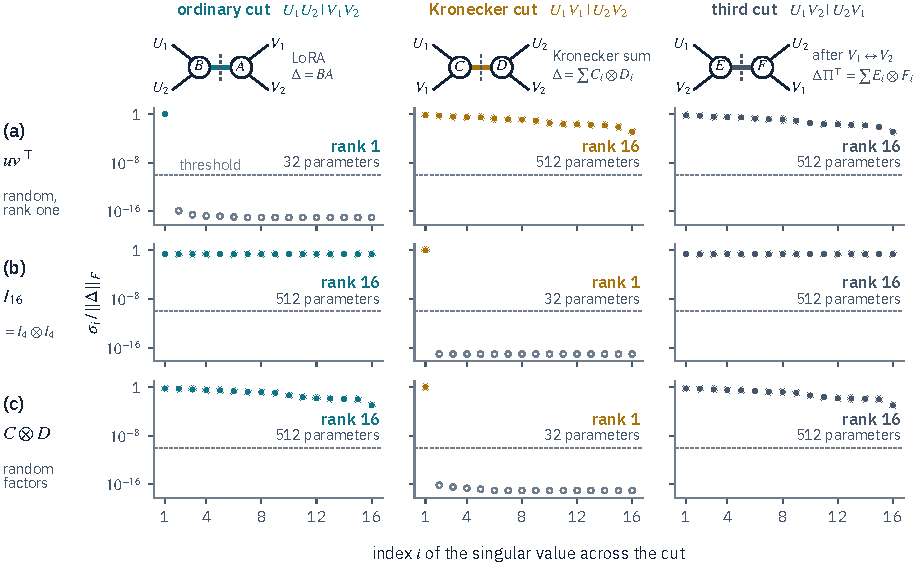
\includegraphics[width=\linewidth]{figures/cut}
  \caption{\textbf{Cut the tensor} (\thmref{Theorem}{II.11}). A $16\times16$ matrix $\Delta$ is read as a four-leg tensor with output legs $U_1,U_2$ and input legs $V_1,V_2$, through $\R^{16}=\R^4\otimes\R^4$ on both sides. The legs can be split into two pairs in three ways (columns): the ordinary cut $\{U_1U_2\}\mid\{V_1V_2\}$, across which LoRA factors as $\Delta=BA$; the Kronecker cut $\{U_1V_1\}\mid\{U_2V_2\}$, across which a sum of Kronecker products $\sum_iC_i\otimes D_i$ factors after the rearrangement of Van Loan and Pitsianis~\citeyearpar{loan1993approximation}; and the third cut $\{U_1V_2\}\mid\{U_2V_1\}$, the Kronecker cut with the two input legs swapped. The glyph above each column draws that factorisation as two boxes joined by a bond across the cut. Each panel shows the operator-Schmidt spectrum across one cut, the singular values $\sigma_i$ of the corresponding $16\times16$ reshape of $\Delta$ divided by $\lVert\Delta\rVert_F$, on a logarithmic scale, for (a)~a random rank-one update $uv\T$, (b)~the identity $I_{16}=I_4\otimes I_4$, and (c)~$C\otimes D$ with random $4\times4$ factors. Filled markers lie above the rank threshold (dashed line), and open markers are numerically zero. The ranks are $(1,16,16)$ for $uv\T$ and $(16,1,16)$ for $I_{16}$ and for $C\otimes D$. So a generic rank-one update has the maximal Kronecker rank $\kappa_1=16$, and a Kronecker product of full-rank factors has the maximal rank $\nu=16$, which makes zero-init LoRA$_r$ and $k$-term Kronecker sums incomparable for $r,k<16$ (\thmref{Theorem}{II.11}(b)--(d)). LoRA$_1$ fits $uv\T$ with $32$ parameters where a Kronecker sum needs $16$ terms and $512$ parameters, and for $I_{16}$ and $C\otimes D$ the two costs trade places.}
  \label{fig:cut}
\end{figure}

% ----------------------------------------------------------------------------------------------------------------------
\subsubsection{Dimension is a volume}\label{sec:cut-volume}

Moving $q\in Q$ along a fibre of $\rho$ changes nothing. For LoRA, $(Bg^{-1},gA)$ gives the same weight as $(B,A)$ for
every $g\in\GL_r$, so $r^2$ of the $r(m+n)$ parameters are spent on a symmetry and the image has dimension $r(m+n-r)$.
This is the expressive dimension $d(M)$ of \thmref{Definition}{I.5}, and $\lvert M\rvert-d(M)$ is the gauge waste.
``Gauge'' means the symmetry group of a parametrisation (\bgref{D.21}). There is no connection, and away from the
full-rank stratum the fibres jump in dimension.

\paragraph{Credit}
The quotient $(\R^{m\times r}_*\times\R^{r\times n}_*)/\GL_r$ is the classical geometry of fixed-rank matrices
\citep{mishra2012fixed}. \citet{putterman2024learning} build learners on LoRA weights that respect this $\GL_r$ symmetry.

The census below covers LoRA \citep{hu2021lora}, GraLoRA \citep{jung2025gralora}, LoHa \citep{hyeonwoo2021fedpara}, HRA
\citep{yuan2024bridging}, DoRA \citep{liu2024dora}, VeRA \citep{kopiczko2023vera}, KronA \citep{edalati2022krona},
tensor-train and Tucker adapters (\bgref{B.9}), and the linear methods LoRA-FA \citep{zhang2023lora}, LoRA-XS
\citep{baazy2024lora}, MiSS \citep{kang2024miss}, FourierFT \citep{gao2024parameter}, C3A \citep{chen2024parameter} and
masks.

\begin{proposition}{II.12}{gauge census: rank is a cut, dimension is a volume}
\begin{enumerate}[label=(\alph*)]
  \item $d(M)\le\lvert M\rvert-\dim(\text{generic gauge orbit})$, with equality when the gauge acts locally
    transitively on generic fibres.
  \item The values in Table~\ref{tab:census} hold for one $m\times n$ box, with $r\le\min(m,n)$ throughout except for
    VeRA (whose published RoBERTa-base setting has $r=1024>768$). In the LoHa row,
    \begin{equation*}
      F=r_1(m+n-r_1)+r_2(m+n-r_2)-(m+n-1)
    \end{equation*}
    is a proved upper bound for $d$. The gauge column lists the exhibited Lie group. It acts locally transitively on
    generic fibres away from the $mn$ cap, but not where the cap binds; for LoHa at $(m,n,r_1,r_2)=(4,4,2,2)$ the orbit
    has dimension $15$ and the fibre $16$. BitFit does not touch the $m\times n$ box; it is linear in the biases. Hybrid
    GraLoRA (\texttt{hybrid\_r}${}>0$) is not covered by the table. FourierFT is injective only when its sampled
    frequencies contain no conjugate pair $(u,v),(-u,-v)$; otherwise $d=\lvert M\rvert-\#\{\text{pairs}\}$. At LLM sizes
    this is close to $\lvert M\rvert$, but at $768\times768$ with $1000$ frequencies a pair occurs in about half of the
    draws (HF's default seed $777$ gives exactly two pairs there).
  \item \emph{Equal-budget trades.} Assume $2r\le\min(m,n)$, $r^2\le\min(m,n)$ and $2r^2<m+n-1$. LoHa$_{r,r}$ and
    LoRA$_{2r}$ both cost $2r(m+n)$, but LoHa reaches at least $(m+n-1)-2r^2$ \emph{fewer} dimensions (exactly that
    many when $F$ is attained [Num]). For $r\ge3$ it gains rank up to $r^2>2r$ in exchange. For $r\le2$, $r^2\le2r$, so
    $\Im\mathrm{LoHa}_{r,r}\subsetneq\Im\mathrm{LoRA}_{2r}$ and LoHa is strictly dominated. When $2r^2\ge m+n-1$ (still with $2r\le\min(m,n)$) the
    bound no longer separates them, and wherever $F$ is attained LoHa$_{r,r}$ matches or exceeds LoRA$_{2r}$ in
    dimension as well as in rank, for instance at $(m,n,r)=(9,9,3)$, at $r=64$ on $4096\times4096$, and at
    LyCORIS-style $r=32$ on $320$- to $640$-wide layers. GraLoRA$_k$ costs the same as LoRA$_r$, reaches the same
    number of dimensions, and has maximum rank $\min(kr,m,n)$, but caps every block at rank $r/k$. A generic rank-$r$
    update has rank $r$ on every block, so for $k\ge2$ and $kr\le\min(m,n)$ the images of LoRA$_r$ and GraLoRA$_k$ are
    incomparable.
\end{enumerate}
\end{proposition}

\begin{table}[t]
  \centering
  \footnotesize
  \caption{The gauge census of \thmref{Proposition}{II.12}(b) for one $m\times n$ box: budget, exhibited Lie gauge with
    the dimension of its generic orbit, expressive dimension and maximum rank. [Num] marks values checked as float64
    Jacobian ranks (Appendix~\ref{app:repro}); $F$ is defined in \thmref{Proposition}{II.12}(b).}
  \label{tab:census}
  \renewcommand{\arraystretch}{1.15}
  \begin{tabularx}{\linewidth}{@{}>{\raggedright\arraybackslash}p{3.0cm}>{\raggedright\arraybackslash}p{1.6cm}>{\raggedright\arraybackslash}X>{\raggedright\arraybackslash}p{3.2cm}>{\raggedright\arraybackslash}p{2.1cm}@{}}
    \toprule
    \headrow \textbf{method} & \textbf{budget $\lvert M\rvert$} & \textbf{exhibited Lie gauge (orbit dim)} &
      \textbf{$d(M)$} & \textbf{max rank}\\
    \midrule
    LoRA$_r$ & $r(m+n)$ & $\GL_r$ ($r^2$) & $r(m+n-r)$ & $r$\\
    GraLoRA ($k\times k$ blocks, rank $r/k$ each; HF default \texttt{hybrid\_r=0}) & $r(m+n)$ & $\prod\GL_{r/k}$
      ($r^2$) & $r(m+n-r)$ & $\min(kr,m,n)$\\
    LoHa$_{r_1,r_2}$ & $(r_1+r_2)(m+n)$ & $\GL_{r_1}\times\GL_{r_2}\times{}$diagonal torus ($r_1^2+r_2^2+m+n-1$) &
      $\min(mn,F)$ [Num]; $F$ is a proved upper bound & $\min(r_1r_2,m,n)$\\
    HRA$_r$ ($\rk W_0=n$, \texttt{apply\_GS=False}; even $r$ is needed only for HF's identity init) & $rn$ & non-linear;
      fibre dimension $r(r+1)/2$; exhibited Lie gauge $(\R^\times)^r$ & $rn-r(r+1)/2$ (for $r\in\{n-1,n\}$ this is
      $\dim\SO(n)$ [Num]) & $r$\\
    DoRA$_r$ & $r(m+n)+m$ & $\GL_r$ for generic $W_0$ with $(m-r)(n-r)\ge m$; larger otherwise (dimension $6>r^2$ at
      $(m,n,r)=(3,3,2)$, and $r^2+r$ for rank-one $W_0$) & $\min\bigl(mn,\,r(m+n-r)+m\bigr)$ for generic $W_0$
      (\thmref{Proposition}{II.8}) & up to full\\
    VeRA & $m+r$ & $\R^\times$ & $m+r-1$ [Num] & $\min(r,m,n)$\\
    KronA $A\otimes B$ & $m_1n_1+m_2n_2$ & $\R^\times$ & $m_1n_1+m_2n_2-1$ & $\min(m_1,n_1)\cdot{}$\newline$\min(m_2,n_2)$\\
    TT / Tucker (admissible, minimal ranks) & $\sum$ cores & $\prod_e\GL_{r_e}$ & $\lvert M\rvert-\sum_er_e^2$ & up to
      full\\
    linear methods (LoRA-FA, LoRA-XS, MiSS in every HF mode, FourierFT, C3A, masks) & $\lvert M\rvert$ & translations
      by the kernel & rank of the linear map; $=\lvert M\rvert$ when injective & varies\\
    \bottomrule
  \end{tabularx}
\end{table}

\paragraph{Numerical check}
LoHa dimensions $38$, $59$, $93$, $101$ at $(m,n,r)=(8,7,2)$, $(12,10,2)$, $(12,10,3)$, $(20,16,2)$, and $16=mn$ at
$(4,4,2)$, where the formula gives $17$ and $d(\mathrm{LoRA}_4)=16$ too. LoHa$_{3,3}$ against LoRA$_6$: $73$ against
$72$ at $(9,9,3)$. GraLoRA dimensions $48$, $64$, $108$ at $(m,n,r,k)=(8,8,4,2)$, $(12,8,4,2)$, $(12,12,6,3)$; GraLoRA
generic rank $8=kr$ at $(16,16,4,2)$ and $12=\min(m,n)$ at $(12,12,6,3)$ (Appendix~\ref{app:repro}).

\paragraph{Credit}
LoHa is the low-rank Hadamard product of FedPara \citep{hyeonwoo2021fedpara}; GraLoRA is due to \citet{jung2025gralora}.
The Tucker gauge and dimension are due to \citet{xkoch2010dynamical} and \citet{xuschmajew2013geometry}, and the TT case
to \citet{xholtz2012manifolds}, building on \citet{oseledets2011tensor}. The intrinsic-dimension experiments of
\citet{li2018measuring} and \citet{aghajanyan2020intrinsic} measure how many random directions a task needs; $d(M)$
counts the directions a method's image has, a complementary notion.

LoHa$_{r,r}$ maps into LoRA$_{r^2}$ through the face-splitting product (\bgref{B.13}), one of the arrow rules of
Exposé~\ref{sec:atlas}; for $r\le2$ this places LoHa$_{r,r}$ inside LoRA$_{2r}$.

\begin{explains}
Rank is a \emph{cut} invariant and dimension a \emph{volume} invariant, and the literature conflates them. When $r\ge3$
and $2r^2$ is small next to $m+n$, as on LLM projections at the usual ranks, LoHa reaches high rank on a thin, curved
subvariety, because its Hadamard product spends a whole torus on gauge. When $2r^2\ge m+n-1$, as in LyCORIS's usual
Stable Diffusion settings, it matches or exceeds LoRA$_{2r}$ in dimension too. GraLoRA keeps LoRA's dimension and
multiplies the maximum rank by $k$, but caps every block at rank $r/k$. It moves the cut, and the block caps pay for the
higher maximum rank.
\end{explains}

% ----------------------------------------------------------------------------------------------------------------------
\subsubsection{Transport of structure}\label{sec:cut-transport}

An invertible linear change of frame fixing $\theta_0$ carries dimension, gauge, first-order image and degree along,
since they are defined from $\rho$ and its differential (\bgref{A.17}). It carries rank along only when it respects rows
and columns, which the Kronecker rearrangement, Fourier and wavelet frames and the Hadamard rescaling by $W_0$ do not.

\begin{proposition}{II.13}{transport of structure}
For $T\in\GL(\Theta)$ put $\tau_T(\theta)=\theta_0+T(\theta-\theta_0)$ and $T_*M:=(Q,q_0,\tau_T\circ\rho)$.
\begin{itemize}
  \item $T_*$ is a strict automorphism of $\Meth(\Theta,\theta_0)$, with inverse $(T^{-1})_*$. It maps $S_1$ to $T\,S_1$
    and preserves $d$, $g$, the gauge group, the first-order deficit, polynomial degree, the regular or apex type and
    the germ type of the image. It does not preserve rank, and, for the family extension below, it does not preserve the
    covariance group.
  \item $K^{T_*M}=T\,K^M\,T\T$ for every $T$. For any update rule that queries the loss only through
    $q\mapsto L(\rho(q))$, with its own state on $Q$, $T_*M$ trained on $L$ and $M$ trained on $L\circ\tau_T$ have
    identical $q$-trajectories, so their $\theta$-trajectories are conjugate by $\tau_T$. Rules that read
    $\nabla_\theta L$ and solve a least-squares problem on $\Theta$ (LoRA-Pro), and $\theta$-level weight decay or
    clipping, are covered only for orthogonal $T$. Orthogonality of $T$ is exactly the condition for $\tau_T$ to be a
    Frobenius isometry; for rules of the first kind it is needed only to keep the Frobenius spectrum of $K$, or an
    isometry-invariant loss class such as $\lVert\theta-\theta^\star\rVert^2$, unchanged.
  \item Coordinatewise optimizers (SGD, Adam) are also equivariant under coordinate permutations of $Q$. The Kronecker
    identification below needs this, because it composes $\mathcal R^{-1}_*$ with the vec reshape of $Q$.
  \item \emph{Families and rebasing.} For $T$ independent of the base point, define the family extension
    $(T_*M)(\theta):=(Q,q_0,\theta+T(\rho_\theta-\theta))$. For an additive family with fixed shape $C$
    (\thmref{Definition}{I.2}), $T_*M$ is additive with shape $TC$, so transport commutes with rebasing:
    $R_K(T_*M)=\tau_T(R_K(M))$ (\thmref{Theorem}{V.3}(a)). For action-type families this can fail even for $T=2I$,
    because the transported family acts by $I+T(g-I)$. For OFT on $\Theta=\R^{1\times2}$, two cycles of
    $\theta\mapsto\theta(2R-I)$ with $R=\operatorname{rot}(\pi)$ reach $9\theta_0$, outside the transported circle.
    Transports that depend on $\theta_0$ may fail (HiRA below) or may not (LoRA transported by the SVD frame of
    $\theta_0$, since $\Mr$ is $\Ort(m)\times\Ort(n)$-invariant). The covariance group (\thmref{Definition}{II.14}) is a
    property of a family and is compared through this extension.
\end{itemize}
Instances.
\begin{itemize}
  \item \emph{Kronecker family.} An isomorphism of slices over $\Theta'=\R^{m_1n_1\times m_2n_2}$ and over $\Theta$:
    $\sum_{i\le k}C_i\otimes D_i=\mathcal R^{-1}_*\mathrm{LoRA}_k$, with $Q$ reshaped by vec, dynamics included for
    coordinatewise optimizers. KronA with unconstrained factors is $\mathcal R^{-1}_*\mathrm{LoRA}_1$. LoKr is
    $\mathcal R^{-1}_*$ of $\mathrm{LoRA}_1$ with the second factor constrained to $\vect\MM_{\le r'}$ when
    $r'<\max(m_2,n_2)/2$ (HF's switch); otherwise HF's second factor is full and LoKr is KronA. LoKr's
    \texttt{decompose\_both} option also constrains the first factor.
  \item \emph{Linear methods as coordinate subspaces in transported frames.}
  \begin{itemize}
    \item FourierFT: sparse in the real cosine half of the real Fourier frame. With scaling $c$ (default $150$), HF's
      update $\Delta W=c\operatorname{Re}(\operatorname{ifft2}(S))$ is the transport of a mask, with $g=0$, only when the sampled index set has no conjugate pair $(u,v),(-u,-v)$; otherwise $g$ is the
      number of such pairs. Its image lies in the point-symmetric subspace $\Delta W_{j,l}=\Delta W_{-j,-l}$, and the
      frame is orthogonal only up to scale (self-conjugate frequencies have twice the squared norm).
    \item WaveFT: sparse in a wavelet frame, when HF's pad--IDWT--crop map is invertible (plausible for Haar on even
      shapes; unverified for other wavelet families).
    \item C3A: block-circulant. Over $\R$ the frame is given by the powers $P^k$ of the cyclic shift (Gram matrix
      $bI$). Over $\mathbb C$, $\operatorname{circ}(w)=F^{-1}\diag(Fw)F$ for first column $w$, and the real form has
      $2\times2$ rotation--scaling blocks. HF adds a factor $1/\texttt{in\_features}$.
    \item LoRA-XS, SVFT, TinyLoRA: masks or random subspaces in the SVD frame of $W_0$, a $\theta_0$-dependent
      transport.
    \item SHiRA, FISH, Trainable Tokens: masks in the standard frame.
    \item MiSS/Bone in its default (balance) mode: $\Delta W=D(\mathbf 1_g\T\otimes I_r)$, which is LoRA-FA with a
      frozen \emph{summing} projection. Its BAT mode, $\Delta W=\operatorname{blocks}(W_0)\,M+M$ blockwise, is linear in
      the trained block $M$ but depends on $\theta_0$, so it is not additive.
    \item These frame readings of FourierFT and C3A are for \texttt{init\_weights=True}. HF's defaults start off
      $\theta_0$: FourierFT draws its spectrum from $\mathcal N(0,1)$ with scaling $150$ (at $768^2$ with $1000$
      frequencies, $\lVert\Delta W_0\rVert_F\approx4.3$, about $14\%$ of a std-$0.04$ $W_0$), and C3A is
      Xavier-uniform. These are objects with a pointing defect.
  \end{itemize}
  \item \emph{HiRA} $=(D_{W_0})_*\mathrm{LoRA}$ inside the slice at $\theta_0$, when $W_0$ has no zero entries, with
    $D_{W_0}:X\mapsto W_0\odot X$. Because $D_{W_0}$ depends on $\theta_0$, re-based HiRA is not transported ReLoRA. Two
    cycles reach $W_0\odot(J+Z_1)\odot(J+Z_2)$, whose relative update $Z_1+Z_2+Z_1\odot Z_2$ has rank up to
    $\min(2r+r^2,m,n)$, attained, where transported ReLoRA stays at rank $\le2r$.
\end{itemize}
\end{proposition}

\paragraph{Numerical check}
$\lVert K^{T_*M}-TK^MT\T\rVert=2\times10^{-14}$ for a Gaussian $T$. Adam on $T_*M$ with $L$ and on $M$ with $L\circ\tau_T$
agree to $8\times10^{-11}$. Two HiRA cycles give relative-update rank $3$, $8$, $15$ at $r=1,2,3$ ($m=n=30$)
(Appendix~\ref{app:repro}).

\paragraph{Credit}
The transported methods are FourierFT \citep{gao2024parameter}, WaveFT \citep{bilican2025exploring}, C3A
\citep{chen2024parameter}, LoRA-XS \citep{baazy2024lora}, SVFT \citep{lingam2024svft}, TinyLoRA
\citep{morris2026learning}, SHiRA \citep{bhardwaj2024sparse}, FISH \citep{sung2021training}, Trainable Tokens
\citep{team2025trainable}, MiSS \citep{kang2024miss} and HiRA \citep{huang2025hira}; LoRA-Pro is due to
\citet{wang2024lorac}. \citet{si2024see} organise PEFT around the SVD frame of $W_0$, a related unification.

\begin{explains}
``High rank'' claims (MoRA, HiRA, LoKr, C3A, SHiRA, WaveFT) are not $\GL(\Theta)$-invariant, although rank is
$\GL_m\times\GL_n$-invariant. The transports in play ($\mathcal R$, the real Fourier (cosine) frame, $D_{W_0}$) do not
preserve the network function, and \thmref{Theorem}{II.11} shows that KronA and $\mathrm{LoRA}_r$ have incomparable
images when $r<\min(m_1,n_1)\min(m_2,n_2)$ and $\kappa_1>1$. Transport preserves every isomorphism invariant of the
method ($d$, $g$, the gauge group, $\dim S_1$, the deficit, the regular or apex type, the germ type and the degree) and
conjugates its dynamics. Relative to the network's $\GL_m\times\GL_n$ structure it changes, in particular, rank,
covariance, $S_1$ as a subspace, and the image itself. In Figure~\ref{fig:rankvol} HiRA therefore sits at LoRA's height
and at full rank (\thmref{Proposition}{II.9}(a)).
\end{explains}

\paragraph{Prediction}
At matched learning-rate sweeps, the performance gap between a transported method and its source (Kronecker sums against
LoRA; Fourier or wavelet methods against coordinate masks) is explained by how well each image aligns with the task's
update, measured for instance by projecting a full fine-tuning $\Delta W$ onto each image, more than by optimizer effects.

% ----------------------------------------------------------------------------------------------------------------------
\subsubsection{The plug, and a reporting rule}\label{sec:cut-plug}

Cut $W_0$ out of a linear layer and a hole $V\to U$ remains. A weight-space method fills it with a small network of
frozen and trainable boxes, a \emph{plug} (Figure~\ref{fig:loraplug}). Every invariant above is read off the plug: the
budget (\thmref{Definition}{I.2}), the min-cut, the Jacobian rank (\thmref{Definition}{I.5}), the gauges on its wires,
and the merge type, set by whether an activation sits on the path (\thmref{Theorem}{VI.3}). The plug is a weight-space
cousin of the unified view of \citet{he2021unified}, which puts adapters, prefix tuning and LoRA in one design space.

Table~\ref{tab:onebudget} spends one budget three ways on one $4096\times4096$ box (\thmref{Proposition}{II.12}). The
methods differ by at least $8{,}063$ dimensions and by a factor of four in rank. The LoHa row uses the upper bound $F$,
whose equality is checked numerically at small sizes and open in general.

\begin{table}[t]
  \centering
  \footnotesize
  \caption{One $4096\times4096$ box and one budget, $\lvert M\rvert=131{,}072$, spent three ways
    (\thmref{Proposition}{II.12}).}
  \label{tab:onebudget}
  \renewcommand{\arraystretch}{1.12}
  \begin{tabularx}{\linewidth}{@{}lrrrX@{}}
    \toprule
    \headrow \textbf{method} & \textbf{$d(M)$} & \textbf{fibre $\lvert M\rvert-d(M)$} & \textbf{max rank} &
      \textbf{block structure}\\
    \midrule
    LoRA$_{16}$ & $130{,}816$ & $256$ & $16$ & none\\
    GraLoRA, $k=2$ & $130{,}816$ & $256$ & $32$ & each of $4$ blocks has rank $\le8$\\
    LoHa$_{8,8}$ & $\le122{,}753$ & $\ge8{,}319$ & $64$ & none\\
    \bottomrule
  \end{tabularx}
\end{table}

\paragraph{Prediction}
Benchmarks should report $d(M)$ beside $\lvert M\rvert$, with the maximum rank and the cut it refers to. At budgets of a
few thousand parameters, rankings at equal \emph{effective} dimension can change.

A small case shows every readout at once. On an $8\times8$ box, LoHa$_{2,2}$ has $64$ parameters, rank at most $4$,
Jacobian rank $41$ and a gauge orbit of dimension $23=4+4+15$ that fills the fibre. LoRA$_4$ costs the same and reaches
$7$ more dimensions, with LoHa's image strictly inside it (\thmref{Proposition}{II.12}(c), since $2r^2=8<15=m+n-1$). The
plug workbench of the companion site recomputes these invariants in float64 for fifteen presets and for plugs the reader
edits: the budget, the degree, the min-cut bound by brute force over vertex bipartitions beside the rank attained, $d(M)$
as a Jacobian rank, the gauge orbit with each generator checked to lie in $\ker d\rho$, and the merge verdict.

% ----------------------------------------------------------------------------------------------------------------------
\subsubsection{Covariance and descent}\label{sec:cut-covariance}

A method is usually one recipe applied to every pretrained weight. Rename a layer's input basis by $h$ and its output
basis by $g$, so that $W_0$ becomes $gW_0h^{-1}$; the method is covariant under $(g,h)$ if its image moves the same way.

\begin{definition}{II.14}{covariance group}
For a method defined for every $W_0$ (a natural family), the \textbf{covariance group}
$\mathcal G_M\subseteq\GL_m\times\GL_n$ is the largest subgroup with $\Im M(gW_0h^{-1})=g\,\Im M(W_0)\,h^{-1}$. When
the method depends on random frames or on data, the identity is required in distribution, with the data transformed.
$\mathcal G_M$ is the \emph{geometry the method lives in}, in Klein's sense.
\end{definition}

Klein defined a geometry by its group of motions and studied what the group leaves unchanged
\citep{xklein1872vergleichende} (\bgref{D.17}). For group-type methods this reading is a theorem (\S\ref{sec:erlangen}).
For cones such as LoRA's image it is a naming device, and the content is the shape of the image and its covariance group.

LoRA's image $W_0+\Mr$ is covariant under all of $\GL_m\times\GL_n$, since rank ignores bases, while a coordinate mask
has a much smaller group. This matters because networks have symmetries of their own, such as permutations of hidden
neurons, rotations of the residual stream and the query--key gauge of attention, which change the weights and keep the
function.

\begin{observation}{II.15}{descent through function-preserving reparametrisations}
Let $M=\prod_bM_b$ be a box-wise method: each $M_b$ is a member of a natural family with covariance group
$\mathcal G_{M_b}$, and no trainable parameters or random frames are shared across boxes. Let $G_{\mathrm{arch}}$ act on
$\Theta=\prod_b\Theta_b\times\Theta_{\mathrm{frozen}}$, preserving this split and acting on each adapted box by
$W_b\mapsto g_bW_bh_b^{-1}$ with $(g_b,h_b)\in\mathcal G_{M_b}$. Assume $f(g\theta,-)=f(\theta,-)$ on a
$G_{\mathrm{arch}}$-stable set containing $\Im M(\theta_0)$. Then $\Im M(g\theta_0)=g\cdot\Im M(\theta_0)$, and the set
of \emph{functions} reachable by $M$ from $g\theta_0$ equals the set reachable from $\theta_0$. For methods with random
frames, the equality holds in distribution, provided the frames are drawn independently per box. Boxes that share a
frame need a pathwise condition: a law-preserving map $T_{(g,h)}$ on frame space with
$\Im M_b(g_bWh_b^{-1};TF)=g_b\,\Im M_b(W;F)\,h_b^{-1}$ for all $W$ and $F$, with the same $T$ on every box that shares
$F$ (marginal covariance in law, as in \thmref{Definition}{II.14}, is not enough). For data-dependent methods, require
covariance pathwise in the data, and that the box-$b$ data at $g\theta_0$ is the \thmref{Definition}{II.14} transform
under $(g_b,h_b)$ of the data at $\theta_0$. This holds for intertwiner gauges such as hidden-unit permutations,
query--key and value--output head gauges and residual rotations. The statement concerns reachable sets only; training
trajectories and outcomes can still differ, for instance under Adam or non-isotropic initialisations.

Examples of $G_{\mathrm{arch}}$:
\begin{itemize}
  \item hidden-neuron permutations;
  \item the query--key gauge $(W_Q,W_K)\mapsto(gW_Q,g^{-\top}W_K)$ per head. With no positional encoding or an absolute
    one, $g\in\GL_{d_k}$. Under RoPE, $g$ must commute with every RoPE rotation, which leaves the per-frequency $2\times2$
    rotation--scalings $(\mathbb C^\times)^{d_k/2}$, shared across a GQA group. Under partial RoPE on $r$ of the $d_k$
    dimensions the group is $(\mathbb C^\times)^{r/2}\times\GL_{d_k-r}$. Under QK-norm, $g$ must in addition be
    orthogonal when the norm's $\varepsilon>0$ (conformal, $g\in\CO(d_k)$, when $\varepsilon=0$) and satisfy
    $g\T\Gamma_qR_t\Gamma_kg=\Gamma_qR_t\Gamma_k$ for every RoPE rotation $R_t$, where $\Gamma_q,\Gamma_k$ are the gains.
    OLMo~2 normalises $q$ and $k$ across all heads jointly;
  \item a single global orthogonal rotation $Q$ of the residual stream of a pre-norm transformer whose norm gains can all
    be fused into the linear layers they feed, after LayerNorm is converted to RMSNorm (SliceGPT's computational
    invariance; QuaRot's offline rotation). SliceGPT's per-block rotations $Q_\ell$ need extra residual matrices and
    change the architecture. Sandwich and post-sublayer norms (Gemma~2 and~3, OLMo~2) are excluded, because their gains
    cannot be fused and $\diag(\gamma)$ does not commute with $Q$. The comparison is between the gain-fused model and the
    fused-and-rotated model: gain fusion is a diagonal input rescaling outside $G_{\mathrm{arch}}$ that already changes
    PiSSA's split and block OFT's image (\thmref{Proposition}{II.16}), and converting LayerNorm to RMSNorm changes LoRA's
    reachable set on the residual writers.
\end{itemize}
\end{observation}

\paragraph{Numerical check}
A tied rank-one update shared by two boxes violates the conclusion (relative distance up to $0.30$), while independent
per-box LoRA satisfies it. A Haar frame shared by two boxes, each covariant in law, gives a joint statistic of $0.44$ from
$\theta_0$ against $0.81$ from $g\theta_0$. Under RoPE a generic $g\in\GL_8$ changes attention scores by up to $313$, a
RoPE-commuting $g$ by $5\times10^{-14}$ (Appendix~\ref{app:repro}).

\paragraph{Credit}
RoPE is due to \citet{xsu2024roformer}. Residual-stream rotations are the device of SliceGPT \citep{xashkboos2024slicegpt}
and of QuaRot \citep{xashkboos2024quarot}. The architectures with sandwich or post-sublayer norms are Gemma~2
\citep{xgemma2024gemma2}, Gemma~3 \citep{xgemma2025gemma3} and OLMo~2 \citep{xolmo2024furious}.

\begin{explains}
Descent is decided by whether each induced pair $(g_b,h_b)$ lies in $\mathcal G_{M_b}$. For one-sided methods
((IA)$^3$, DoRA, OFT, BOFT) this is a question of side. For coordinate-structured methods (LoHa with $r\ge2$, HiRA, masks,
FourierFT, Kronecker methods) it is a question of group. They descend through hidden-unit monomial gauges, since
$P(X\odot Y)Q=(PXQ)\odot(PYQ)$ for permutation matrices $P,Q$ and a diagonal scaling can be absorbed into one factor, and
they do not descend through rotations. A global residual rotation acts on the input side of $q$, $k$, $v$, gate and up,
and on the output side of $o$ and down.
\end{explains}

Table~\ref{tab:descent} sorts common methods by this criterion. Failing a sufficient condition does not prove that the
reachable function sets differ.

\begin{table}[t]
  \centering
  \footnotesize
  \caption{Methods against the sufficient condition of \thmref{Observation}{II.15}. For the residual rotation the
    comparison is between the gain-fused model and the fused-and-rotated model.}
  \label{tab:descent}
  \renewcommand{\arraystretch}{1.15}
  \begin{tabularx}{\linewidth}{@{}>{\raggedright\arraybackslash}p{2.6cm}>{\raggedright\arraybackslash}X>{\raggedright\arraybackslash}X@{}}
    \toprule
    \headrow \textbf{gauge} & \textbf{satisfy the hypothesis (reachable functions unchanged)} & \textbf{fail the
      sufficient condition}\\
    \midrule
    single global residual rotation (SliceGPT style) & LoRA, full FT, BitFit, PiSSA; (IA)$^3$ with HF defaults, which
      scales the output side of $k$ (or $q$, for Qwen, Gemma and Phi) and $v$ and the input side of down, while the
      rotation acts on the other side, where (IA)$^3$ is $\GL$-covariant; DoRA on $q$, $k$, $v$, gate and up; OFT on $o$
      and down (no scale); LoHa$_1$, whose image is $W_0+\MM_{\le1}$ & block OFT and BOFT on residual-input projections
      (the block normaliser contains no Hadamard or PCA rotation); BOFT on $o$ and down (its output scale
      \texttt{boft\_s}); DoRA on $o$ and down; LoHa with $r\ge2$; HiRA; coordinate masks; FourierFT\\
    query--key and value--output head gauges & LoRA & (IA)$^3$ on $q$ or $k$ and on $v$; OFT on $o$\\
    \bottomrule
  \end{tabularx}
\end{table}

\begin{conjecture}{A}{reachable sets under a residual rotation}
Against a gain-fused but unrotated control, fine-tuning the fused-and-rotated, function-identical model measurably
changes the reachable function sets, and the results, of block OFT/BOFT on residual-input projections, LoHa with
$r\ge2$, HiRA and coordinate masks, because LLM residual streams have a privileged basis.
\end{conjecture}

QuaRot's per-head Hadamard on $W_v$ and $W_{\mathrm{out}}$ is a value--output gauge in $G_{\mathrm{arch}}$. Its online
Hadamards (across heads, before down\_proj, on keys) preserve the realised function but insert new operations, so they
change the architecture map and lie outside $G_{\mathrm{arch}}$. The optimizer adds a further layer. Adam is only
$B_r$-equivariant (\thmref{Theorem}{III.12}) and HF's Kaiming-uniform $A$ is not rotation-invariant in law, so LoRA
\emph{trained with Adam} need not descend even though its image does.

% ----------------------------------------------------------------------------------------------------------------------
\subsubsection{Covariant data-aware splits}\label{sec:cut-splits}

SVD-based initialisations raise the same question. PiSSA, MiLoRA and CorDA split $W_0$ into a trainable part and a
frozen residual by a truncated SVD of $W_0$ or, for CorDA, of $W_0$ weighted by the input second moment. Truncated SVD
commutes only with rotations and uniform scalings, so these splits depend on the input coordinates, and whitening
removes that dependence.

\begin{proposition}{II.16}{covariant data-aware splits}
Let $C=\mathbb E[xx\T]\succ0$ be the input second moment, so that under $x\mapsto hx$ we have $W\mapsto Wh^{-1}$ and
$C\mapsto hCh\T$. Let $LL\T=C$ and $p:=\min(m,n)$. Write $[M]_r$ for the rank-$r$ truncated SVD,
$\langle M\rangle_r:=M-[M]_{p-r}$ for the bottom $r$ singular components, and $\CO(n)=\R_{>0}\cdot\Ort(n)$. Assume
$1\le r<p$ and the spectral gap each split needs: $\sigma_r>\sigma_{r+1}$ of $W_0L$ in (a); in (b),
$\sigma_r>\sigma_{r+1}$ of $W_0C$ or $W_0$ for top-$r$ splits, and $\sigma_{p-r}>\sigma_{p-r+1}$ for bottom-$r$ splits.
Covariance groups are taken over the generic set where these gaps hold.

(a) The whitened split
\begin{equation*}
  X^*=\arg\min_{\rk X\le r}\lVert(W_0-X)L\rVert_F=[W_0L]_rL^{-1}=\Pi_rW_0,
\end{equation*}
where $\Pi_r$ is the top-$r$ eigenprojector of the output second moment $W_0CW_0\T$, is $\GL_n$-covariant on the input
side and $\CO(m)$-covariant on the output side; its joint group is $\CO(m)\times\GL_n$. This is the classical
reduced-rank-regression (SVD-LLM) solution.

(b) The formula-level CorDA splits, IPM ($X=[W_0C]_rC^{-1}$, the minimiser of $\lVert(W_0-X)C\rVert_F$) and KPM (the
bottom-$r$ components of $W_0C$ mapped back by $C^{-1}$, $X=\langle W_0C\rangle_rC^{-1}$), with or without CorDA's
trace-relative damping $C+\kappa(\tr C/n)I$, and the PiSSA and MiLoRA splits ($[W_0]_r$ and the bottom-$r$ part
$\langle W_0\rangle_r$), have input-side covariance group exactly $\CO(n)$; jointly, $\CO(m)\times\CO(n)$.

(c) \emph{Scope.} An absolute damping $C+\lambda I$ reduces the input-side group of (a) and of (b) to $\Ort(n)$. The
official and HF CorDA code divide each calibration sample by the absolute value of its largest entry before
accumulating $C$, which keeps only positive scalings and coordinate permutations, so (b) describes the CorDA formulas and
does not cover shipped CorDA under rotations.
\end{proposition}

\paragraph{Numerical check}
Under $h=3Q$ with $Q$ orthogonal, CorDA (IPM and bottom-$r$ KPM), PiSSA and bottom-$r$ MiLoRA move covariantly to
$4\times10^{-15}$. Under a generic $h$ only the whitened split does ($2\times10^{-15}$, against $0.63$ and $1.1$). At
$r=n$ PiSSA is $\GL_n$-covariant. An absolute damping $0.1$ breaks the whitened split under a generic $h$ ($0.14$), and
under $h=3Q$ (about $2\times10^{-2}$), while trace-relative damping keeps it ($3\times10^{-15}$)
(Appendix~\ref{app:repro}).

\paragraph{Credit}
The splits are CorDA \citep{yang2024corda}, PiSSA \citep{meng2024pissa} and MiLoRA \citep{wang2024milora}. The whitened
truncation is the one used by SVD-LLM \citep{xwang2025svdllm} for compression.

\begin{explains}
A design rule from the Erlangen programme. A sufficient condition for a data-aware Type~II split to be independent of how
a layer's input coordinates are chosen is that it be a left multiple of $W_0$ by a matrix-valued function of the output
second moment, $X=\Phi(W_0CW_0\T)\,W_0$. The whitened (SVD-LLM-style) split and the eigenprojector split of Astra
\citep{liu2026astra} are instances; Astra's paper form, a tail eigenprojector of the output covariance, has the same form
with $C$ replaced by the centred input covariance, which transforms in the same way. Depending on the data only
through $W_0CW_0\T$ is not enough, since PiSSA satisfies that vacuously and is not $\GL_n$-covariant. Non-conformal
reparametrisations, such as the diagonal rescalings from norm-gain folding or SmoothQuant \citep{xxiao2023smoothquant},
change the CorDA and PiSSA splits.
\end{explains}

Three caveats apply. An absolute damping $C+\lambda I$ reduces the covariance to $\Ort(n)$, while CorDA's trace-relative
damping keeps $\CO(n)$. The covariance is one-sided. No rank-$r$ split that depends only on $(W_0,C)$ can be
$\GL_m\times\GL_n$-covariant, since the stabiliser of a normal form contains an orthogonal group that fixes only
full-rank or zero splits, and whitening with the output second moment itself is degenerate (every singular value of
$(W_0CW_0\T)^{-1/2}W_0L$ is $1$). Descent through hidden-layer $\GL$ gauges would need an output-side statistic
independent of $(W_0,C)$, such as a backpropagated-gradient second moment. Training dynamics (SGD, Adam) remain
non-covariant.

EVA \citep{paischer2024parameter} is not a split. It is Type~I ($B_0=0$, $W_0$ not split) and points
$\operatorname{row}A_0$ at the top-$r$ centred principal subspace of the inputs. At a fixed rank its image $W_0+\Mr$ is
$\GL_m\times\GL_n$-covariant under \thmref{Definition}{II.14}, and only its pointing $\operatorname{row}A_0$ is
$\CO(n)$-covariant. With HF's default \texttt{rho=2.0} the per-layer rank is redistributed by explained-variance ratios,
which are only $\CO(n)$-invariant, so the image becomes $\GL_m\times\CO(n)$-covariant.

\begin{conjecture}{C}{whitened splits}
Whitened CorDA or PiSSA is more robust to function-preserving input reparametrisations, and no worse otherwise.
\end{conjecture}

Rank is a cut, dimension a volume and covariance a group. All three can be computed before training. The next exposé
turns from what a method can reach to how it moves there.
